\documentclass[crop=false]{standalone}
\usepackage{standard}

\begin{document}
  \section{Grundlagen und der naive Algorithmus} % (fold)
  \label{sub:naiver_algorithmus}
    Abbildung \ref{fig:raytracing} stellt eine Skizze des grundsätzlichen Algorithmus dar.
    Für jeden Pixel des Pixelpuffers wird ein Strahl von der Kameraposition durch den Pixel in die Richtung des Bildschirms ausgesendet.
    Jeder dieser Strahlen wird dann mit der Szene auf Schnittpunkte getestet.
    Existiert ein Schnittpunkt, so wird dieser durch weitere Algorithmen dargestellt.
    Existieren mehrere Schnittpunkte, so wird derjenige ausgewählt, der der Kamera am nächsten ist.
    \begin{figure}[h]
      \center
      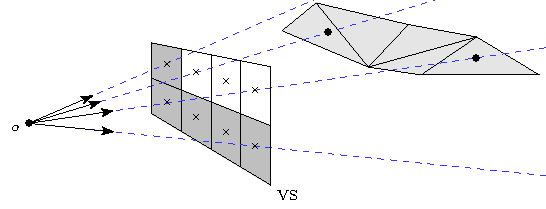
\includegraphics[width=0.8\textwidth]{images/ray_tracing_scheme.pdf}
      \caption{%
        Die Skizze stellt das Raytracing-Verfahren dar.
        Bezüglich eines Beobachtungspunktes $o$ wird durch jeden Pixel eines virtuellen Bildschirms $\mathrm{VS}$ ein Strahl geschossen.
        Die grau melierten Dreiecke stellen dabei die Szene dar.
        Jeder Pixel des virtuellen Bildschirms entspricht einem analogen Pixel des realen Bildschirms.
      }
      \label{fig:raytracing}
    \end{figure}

    \subsection{Aufbau der Kamera} % (fold)
    \label{sub:aufbau_der_kamera}
      Für die Implementierung wurde das Einlesen der Szene als Liste von Dreiecken wie in Abschnitt \ref{ssub:einlesen_der_daten} realisiert.
      Die Kamera konnte mithilfe einer Klasse dargestellt werden.
      In der folgenden Abbildung \ref{fig:camera-scheme} ist die Bedeutung der einzelnen Parameter skizziert.
      \begin{figure}[h]
        \center
        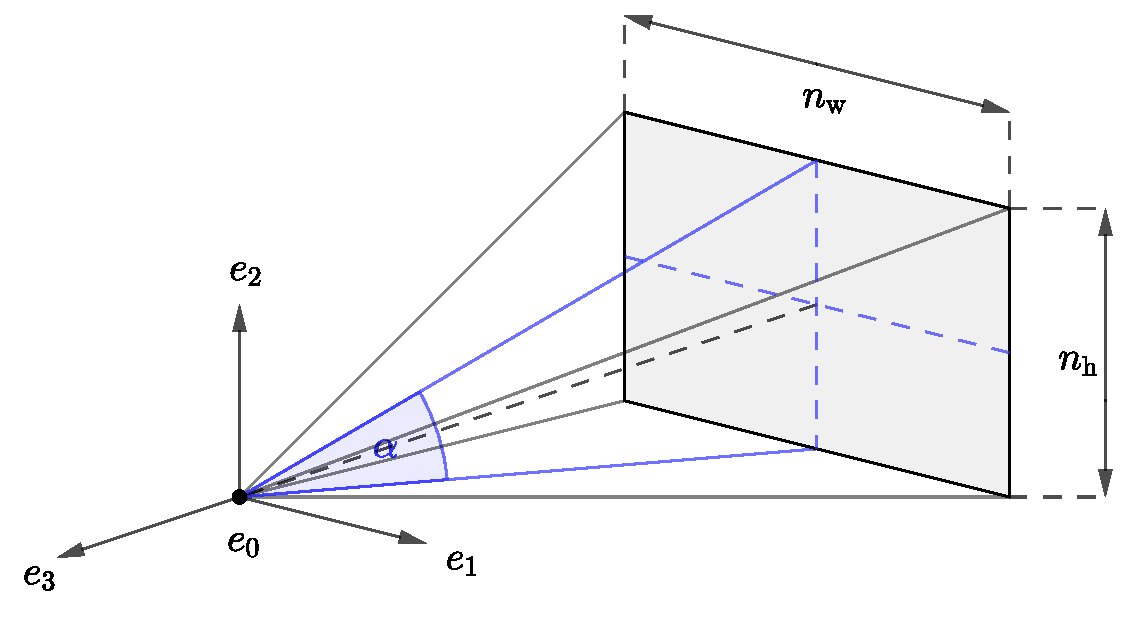
\includegraphics[width=0.8\textwidth]{images/camera_scheme.pdf}
        \caption{%
          Die Abbildung veranschaulicht die Parameter der Klasse \texttt{Camera} anhand einer Skizze.
          Das Tupel $\roundBrackets{e_0,\set{e_1,e_2,e_3}{}}$ beschreibt die affine Basis, $n_\mathrm{w}$ und $n_\mathrm{h}$ die Breite und die Höhe des virtuellen Bildschirms in Pixeln und $α$ den Öffnungswinkel (engl.: \textit{field of view}).
        }
        \label{fig:camera-scheme}
      \end{figure}
      Die Position und Ausrichtung der Kamera wurde durch eine positiv orientierte affine Basis im $\setReal^3$ beschrieben.
      Der erste Basisvektor zeigt in die Richtung, die für die Kamera als rechts definiert ist.
      Analoges gilt für den zweiten und dritten Basisvektor bezüglich den Richtungen oben und hinten.
      Der zu einer Kamera gehörige virtuelle Bildschirm wurde durch die Anzahl seiner Pixel $n_\mathrm{w}$ und $n_\mathrm{h}$ in der Breite und Höhe charakterisiert.
      Die Entfernung zur Kamera wurde durch den Öffnungswinkel $\alpha$ (engl.: \textit{field of view}), unter dem die Höhe des Bildschirms von der Kamera aus zu sehen ist, angegeben.
      Weitere Größen wie die Kantenlänge $p$ eines Pixels im Raum oder das Seitenverhältnis $r$ des virtuellen Bildschirms lassen sich aus den bereits definierten Größen eindeutig berechnen.
      \[
        p = \frac{2\tan \frac{\alpha}{2}}{n_\mathrm{h}}
        \qquad
        r = \frac{n_\mathrm{w}}{n_\mathrm{h}}
      \]
    % subsection aufbau_der_kamera (end)

    \subsection{Strahl-Dreieck-Schnittpunkttest} % (fold)
    \label{sub:strahl_dreieck_schnittpunkttest}
      Die von der Kamera ausgesendeten Primärstrahlen mussten auf Schnittpunkte mit der Szene getestet werden.
      Für jeden Strahl wurden hierfür mithilfe des Möller-Trumbore-Verfahrens die Schnittpunkte mit allen Dreiecken der Szene berechnet.
      Um das genannte Verfahren genauer zu erklären, seien $A,B,C\in \setReal^3$ die Eckpunkte eines Dreiecks, wobei gilt, dass die Menge $\left\{ B-A,C-A \right\}$ linear unabhängig ist.
      Wie sich leicht überprüfen lässt, lassen sich alle Punkte des Dreiecks durch die folgende Parametrisierung beschreiben.
      \begin{align*}
        &M \define \set{ (u,v)\in [0,1]^2 }{ u+v \leq 1 } \\
        &\function{\varphi}{M}{\mathds{R}^3}
        \separate
        \varphi(u,v)\define (1-u-v)A + uB + vC
      \end{align*}
      Die Koordinaten $u$, $v$ und $1-u-v$ werden auch als die baryzentrischen Koordinaten eines Dreiecks bezeichnet.
      Weiterhin nehmen wir an, dass ein Strahl durch die folgende Funktion $r$, den Ursprung $o\in\mathds{R}^3$ und die Richtung $d\in\mathds{R}^3\setminus\{0\}$ beschrieben wird.
      \[
        \function{r}{[0,\infty)}{\mathds{R}^3}
        \separate
        r(t) \define o + td
      \]
      Für einen Schnittpunkt zwischen Strahl und Dreieck muss die folgende Gleichung für $(u,v)\in M$ und $t\in[0,\infty)$ erfüllt sein.
      \[
        r(t) = φ(u,v)
      \]
      Zur Lösung dieser Gleichung setzt man zunächst die Parametrisierungen von Strahl und Dreieck ein.
      \[
        o + td = A + (B-A)u + (C-A)v
      \]
      Durch Umbenennung der konstanten Vektoren lässt sich diese Gleichung in einer übersichtlicheren Form darstellen.
      Abbildung \ref{fig:ray-triangle-intersection-scheme} skizziert die Bedeutung aller bisher verwendeten Variablen.
      \[
        e_0 = ue_1 + ve_2 - td
      \]
      \[
        e_0 \coloneqq o - A
        \qquad
        e_1 \coloneqq B-A
        \qquad
        e_2 \coloneqq C-A
      \]
      \begin{figure}[h]
        \center
        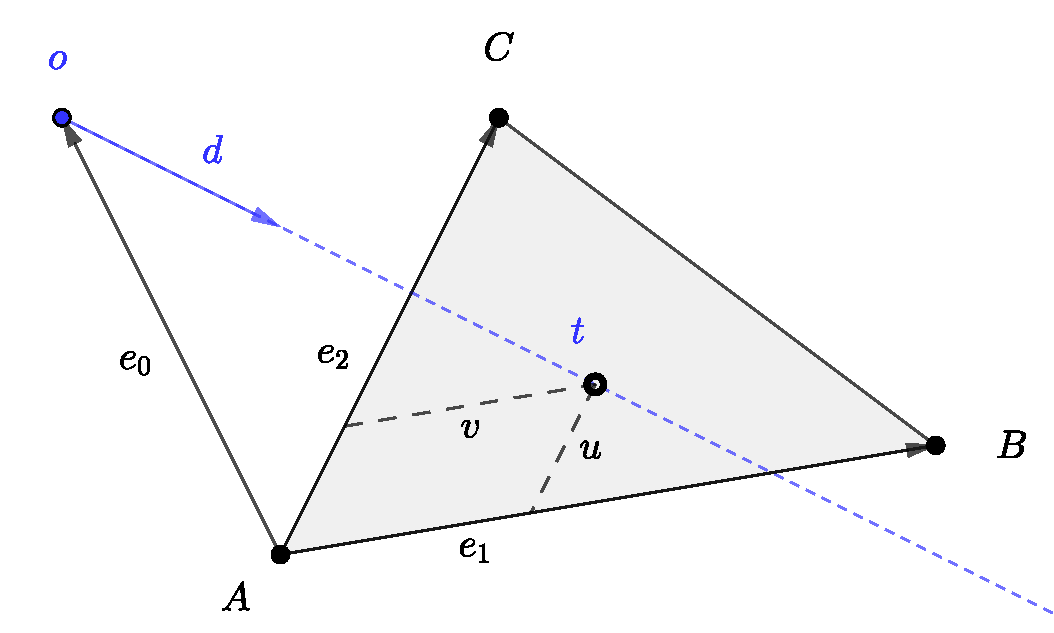
\includegraphics[width=0.6\textwidth]{images/ray_triangle_intersection_scheme.pdf}
        \caption{%
          Die Abbildung zeigt die Bedeutung der verwendeten Variablen der Schnittpunktberechnung zwischen Strahl und Dreieck anhand einer Skizze.
        }
        \label{fig:ray-triangle-intersection-scheme}
      \end{figure}

      Fasst man nun die Koordinaten $u$, $v$ und $t$ zu einem Vektor zusammen, so lässt sich die Gleichung sehr elegant durch ein Matrix-Vektor-Produkt formulieren.
      Hierbei gehen wir davon aus, dass es sich bei den Vektoren $e_0$, $e_1$, $e_2$ und $d$ um Spaltenvektoren handelt.
      \[
        e_0 =
        \begin{pmatrix}
          e_1 &
          e_2 &
          -d
        \end{pmatrix}
        \begin{pmatrix}
          u \\
          v \\
          t
        \end{pmatrix}
      \]
      Der Schnittpunkt zwischen einem Strahl und einem Dreieck kann demnach aus der Lösung eines linearen Gleichungssystems, charakterisiert durch eine $3\times 3$-Matrix, gewonnen werden.
      Offensichtlich wird die Determinante der angegebenen Matrix genau dann Null, wenn der Strahl parallel zur Ebene des Dreiecks verläuft.
      % Dieses lineare Gleichungssystem ist genau dann lösbar, wenn die Determinante der Matrix ungleich Null ist.
      In diesem Falle existieren entweder keine oder unendlich viele Schnittpunkte, sodass keine Aussagen über $u$, $v$ und $t$ getroffen werden können.
      Nimmt man nun an, dass die Matrix nicht singulär ist, so lässt sich die Gleichung durch eine Invertierung lösen.
      \[
        \begin{pmatrix}
          u \\
          v \\
          t
        \end{pmatrix}
        =
        \begin{pmatrix}
          e_1 &
          e_2 &
          -d
        \end{pmatrix}^{-1}
        e_0
      \]
      Die Inverse der Matrix lässt sich analytisch leicht durch Skalar- und Kreuzprodukte beschreiben.
      Innerhalb des Computers ermöglicht diese Formulierung zudem eine effizientere Auswertung der Schnittpunkte.
      \[
        \begin{pmatrix}
          u \\
          v \\
          t
        \end{pmatrix}
        =
        \frac{1}{\left\langle e_1, d\times e_2  \right\rangle}
        \begin{pmatrix}
          \left\langle d\times e_2 , e_0 \right\rangle \\
          \left\langle e_1\times d , e_0 \right\rangle \\
          \left\langle e_1\times e_2, e_0 \right\rangle
        \end{pmatrix}
      \]
      In einem letzten Schritt werden die Vektoren innerhalb der Skalar- und Kreuzprodukte zyklisch vertauscht, um die Lösung der Gleichung nur durch die Berechnung von zwei verschiedenen Kreuzprodukten zu erhalten.
      \[
        \begin{pmatrix}
          u \\
          v \\
          t
        \end{pmatrix}
        =
        \frac{1}{\left\langle e_1, d\times e_2  \right\rangle}
        \begin{pmatrix}
          \left\langle d\times e_2 , e_0 \right\rangle \\
          \left\langle e_0\times e_1 , d \right\rangle \\
          \left\langle e_0\times e_1, e_2 \right\rangle
        \end{pmatrix}
      \]
      Durch diese Gleichung lassen sich nun die Parameter $u$, $v$ und $t$ eindeutig bestimmen.
      Abschließend muss überprüft werden, ob diese auch die Bedingungen der Parametrisierungen $(u,v)\in M$ und $t\in [0,\infty)$ erfüllen.
      Die folgenden Ungleichungen stellen diese in vereinfachter Form dar.
      \[
        \left\langle e_1, d\times e_2  \right\rangle \neq 0
        \qquad
        u,v,t \geq 0
        \qquad
        u+v\leq 1
      \]
      Sind die Bedingungen erfüllt, so liegt ein Schnittpunkt vor.
      Eine beispielhafte Implementierung ist in dem folgenden Quelltext zu sehen.

      \inputCodeBlock[title=Möller-Trumbore-Algorithmus]{code/moeller_trumbore_intersection.cc}
    % subsection strahl_dreieck_schnittpunkttest (end)
  % section naiver_algorithmus (end)
\end{document}